
\chapter{Sistemas Fotovoltaicos de Bombeo\label{cha:SFB}}




\section{Conceptos generales}

Un sistema fotovoltaico de bombeo (SFB) emplea un generador fotovoltaico
para alimentar una motobomba y extraer agua de un pozo, almacenarla
en un depósito o transportarla de un lugar a otro.  \nomenclature[SFB]{SFB}{Sistema fotovoltaico de bombeo} 

Esta aplicación de la tecnología fotovoltaica posee dos peculiaridades
que la hacen particularmente atractiva. En primer lugar, las curvas
de generación y de consumo están bien adaptadas: las épocas de mayor
radiación solar y consiguiente productividad eléctrica son a la vez
las de mayor consumo de agua. En segundo lugar, no es necesario emplear
acumuladores electroquímicos para almacenar energía y dotar de autonomía
al sistema: un depósito elevado de agua almacena energía potencial
de forma más barata, segura, eficiente y fiable. Se habla entonces
de un sistema fotovoltaico de bombeo directo (SFBD). Dado que el empleo
de depósitos de agua como medio de acumulación es, con diferencia,
la configuración más extendida, a lo largo de este capítulo obviaremos
esta distinción.


\section{Componentes}

La figura \ref{fig:ComponentesSFB} muestra los principales componentes
de un SFB: el generador fotovoltaico, la motobomba, el equipo de acoplamiento
entre generador y motobomba, el circuito hidraúlico y el depósito
de agua. Se recogen a continuación las características principales
de cada uno de ellos.

%
\begin{figure}
\begin{centering}
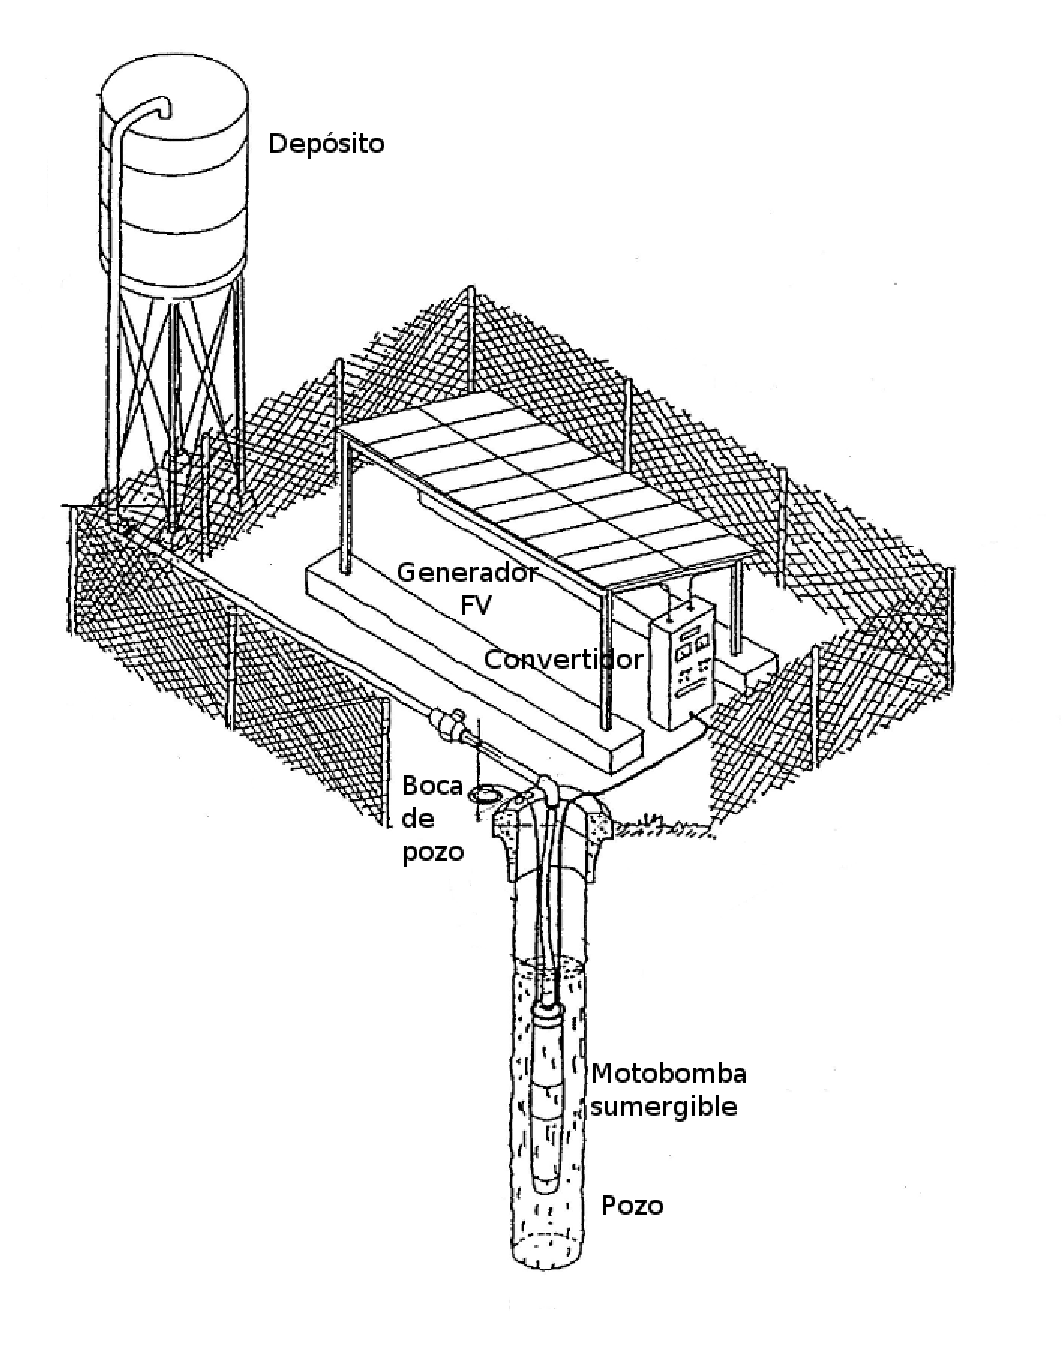
\includegraphics[scale=0.5]{../figs/EsquemaBombeo_oscar}
\end{centering}

\caption[Componentes de un sistema fotovoltaico de bombeo de agua.]{\label{fig:ComponentesSFB} Componentes de un sistema fotovoltaico
de bombeo de agua. Adaptado de \cite{Lorenzo.Narvarte2006}.}

\end{figure}



\subsection{Motobomba}

En sistemas fotovoltaicos es frecuente el empleo de motobombas, equipos
que integran de forma conjunta un motor eléctrico que acciona la bomba
de agua. Veamos el funcionamiento de un motor eléctrico y de una bomba
de agua. 


\subsubsection{Motores eléctricos}

Un motor eléctrico es una máquina eléctrica que transforma energía
eléctrica en energía mecánica por medio de interacciones electromagnéticas.
Repasemos brevemente algunos conceptos fundamentales de electromagnetismo
que nos servirán para comprender el funcionamiento de los motores
eléctricos. 

Desde la experiencia de Oersted es sabido que una corriente eléctrica
crea un campo magnético en torno al conductor que la transporta. Además,
según la ley de Lorentz, un campo magnético ejerce una fuerza sobre
una carga eléctrica en movimiento. Así, un conductor por el que circula
corriente, situado en el seno de un campo magnético, altera este campo
magnético al crear uno nuevo, y dado que la corriente es carga eléctrica
en movimiento, experimenta una fuerza que lo expulsa para disminuir
la alteración (fuerza de Ampere).

Por otra parte, tal y como describe la ley de inducción electromagnética
de Faraday, entre los puntos extremos de una espira atravesada por
un campo magnético, aparece una tensión inducida siempre que el flujo
magnético sea variable. Esta condición se cumple cuando la espira
está en movimiento, cuando el campo magnético es variable, o cuando
ambas situaciones coinciden. La tensión inducida es directamente proporcional
a la rapidez con que cambia en el tiempo el flujo magnético que atraviesa
la superficie encerrada por la espira. Al elemento que emite el campo
magnético se le denomina inductor y aquel que es atravesado por este
flujo es el inducido. 

Si la espira se cierra, circulará una corriente que, a su vez, creará
un campo magnético que contrarrestará la variación de flujo. Además,
al circular corriente, el campo magnético primero realizará una fuerza
sobre la espira en forma de par de giro. Este par de giro es el resultado
aprovechable del motor en forma de potencia mecánica. Este par busca
restablecer el equilibrio existente antes de la introducción de la
espira en el campo magnético intentando alinear los ejes magnéticos
de inductor e inducido. Una vez que están alineados, el par es nulo
y el motor cesa su movimiento. Por esta razón, los diferentes tipos
de motor incorporan un mecanismo para evitar que se produzca este
equilibrio. En la terminología de motores, el elemento que permanece
fijo es el estator y el que realiza el giro es el rotor. Según el
tipo de motor, el rotor puede ser el inducido y el estator el inductor
o viceversa. 

La relación entre las frecuencias eléctricas en inductor e inducido
y la velocidad de giro del rotor es:

\begin{eqnarray}
f_{2} & = & f_{1}-n\cdot p\label{eq:FrecuenciaMotor}\end{eqnarray}
siendo $f_{2}$ la frecuencia en el inducido, $f_{1}$ la frecuencia
en el inductor, $n$ la velocidad angular y $p$ el número de pares
de polos%
\footnote{Una máquina bipolar ($p=1$) utiliza en el inductor un circuito magnético
con dos polos, Norte y Sur. En esta máquina, el ángulo magnético y
geométrico coinciden. En máquinas multipolares ($p>1$) el inductor
está constituido por un circuito magnético con pares Norte-Sur que
se van sucediendo. En este caso, al realizar el giro completo se recorren
varios ciclos magnéticos de forma que a un ángulo magnético, $\theta$,
le corresponde un ángulo geométrico, $\alpha$, según la relación
$\theta=p\cdot\alpha$.%
}. Aquellos motores que emplean un colector de delgas (escobillas)
en el inducido modifican la frecuencia en el circuito exterior, $f_{L}$,
y por tanto $f_{L}\neq f_{2}$. En base a la ecuación \ref{eq:FrecuenciaMotor}
se establecen las categorías de motores. Los dos motores más empleados
en los SFB son el motor de continua y el motor de inducción.

El motor de continua emplea un estator-inductor alimentado por corriente
DC (o imanes permanentes), alimentando el rotor-inducido mediante
una corriente DC transformada en alterna con un colector de delgas.
De esta forma, el giro del rotor está sincronizado con la frecuencia
de la corriente transformada. En este motor se cumple $f_{1}=0$;
$f_{L}=0$; $f_{2}=np$. El uso de escobillas somete a estos motores
a un desgaste que obliga a su mantenimiento. Por esta razón, no están
indicados para su empleo con bombas sumergidas. No obstante, existen
motores DC sin escobillas, donde la conmutación se realiza mediante
un circuito electrónico. Los motores de escobillas no necesitan inversor,
tienen buen rendimiento, pero están indicados para potencias bajas.

El motor asíncrono o de inducción emplea un estator-inductor alimentado
por una corriente trifásica alterna que produce un campo magnético
giratorio. El rotor-inducido está constituido por espiras cortocircuitadas
(jaula de ardilla). Con esta configuración, se produce un par mecánico
que busca alinear el eje de las espiras con el campo giratorio consiguiendo
que el rotor se mueva siguiendo al campo. En este motor se cumple
$f_{1}\neq0$; $f_{L}=f_{2}=f_{1}-np$. Por tanto, la velocidad de
giro es inferior a la frecuencia de alimentación, lo que confiere
a este motor el nombre de asíncrono.

Este tipo de motores son los más comunes y en muchos casos más baratos
que los de corriente continua. Tienen pares de arranque muy bajos,
adecuados para bombas que requieren bajo par de arranque, como las
centrífugas. Requieren el uso de un equipo denominado variador de
frecuencia para adaptar las condiciones de trabajo del generador a
las del motor. 


\subsubsection{Bombas hidráulicas}

Una bomba es una máquina hidráulica que transforma la energía mecánica
con la que es accionada en energía hidráulica del fluido (agua en
el caso de los SFB). Al incrementar la energía del fluido, se aumenta
su presión, su velocidad o su altura, todas ellas relacionadas con
la conservación de la energía expresada en el principio de Bernoulli
(ecuación \ref{eq:Bernouilli}). Cada tipo de bomba altera uno de
estos factores para transportar el agua. 

\begin{equation}
\frac{\Delta p}{\rho}+\frac{\Delta v^2}{2}+g\cdot\Delta h=cte.\label{eq:Bernouilli}\end{equation}
siendo $p$ la presión, $\rho$ la densidad del fluido, $v$ la velocidad,
$g$ la gravedad y $h$ la altura.

Las \emph{bombas de desplazamiento positivo} tienen como principio
el aumento de presión. Están formadas por un contorno móvil que obliga
al fluido a avanzar por la máquina por cambios de volumen. Son apropiadas
para altos incrementos de presión y bajos caudales. Necesitan un elevado
par de arranque (por tanto, no pueden ser acopladas directamente al
generador).

Se pueden distinguir entre:
\begin{itemize}
\item \emph{Bombas de émbolo alternativo}, en las que existe uno o varios
compartimentos fijos, pero de volumen variable, por la acción de un
émbolo o de una membrana (figura \ref{fig:Bomba-de-diafragma}). Son
destacables las \emph{bombas de diafragma}, más económicas, pero que
requieren el reemplazo de los diafragmas cada dos o tres años, dependiendo
del fabricante.
\item \emph{Bombas volumétricas}, en las que una masa fluida es confinada
en uno o varios compartimentos que se desplazan desde la zona de entrada
(de baja presión) hasta la zona de salida (de alta presión) de la
máquina. En los SFB es frecuente el uso de las denominadas \emph{bombas
helicoidales} (figura \ref{fig:Bomba-helicoidal}).
\end{itemize}
%
\begin{figure}
\begin{centering}
\hfill{}\subfloat[]{\begin{centering}
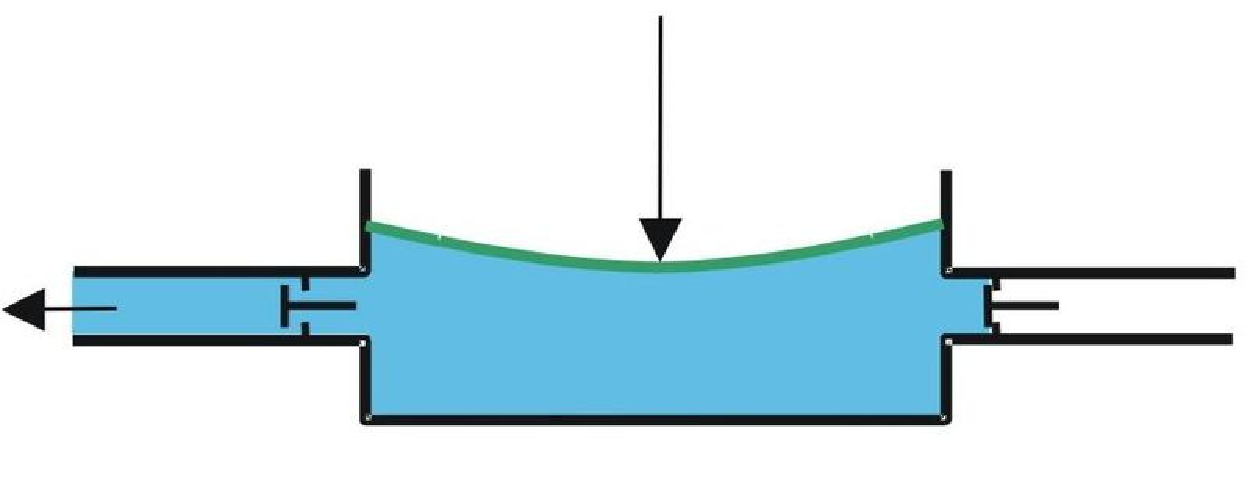
\includegraphics[scale=0.3]{../figs/800px-Bomba_diafragma_impulsando}
\par\end{centering}

}\hfill{}\subfloat[]{\begin{centering}
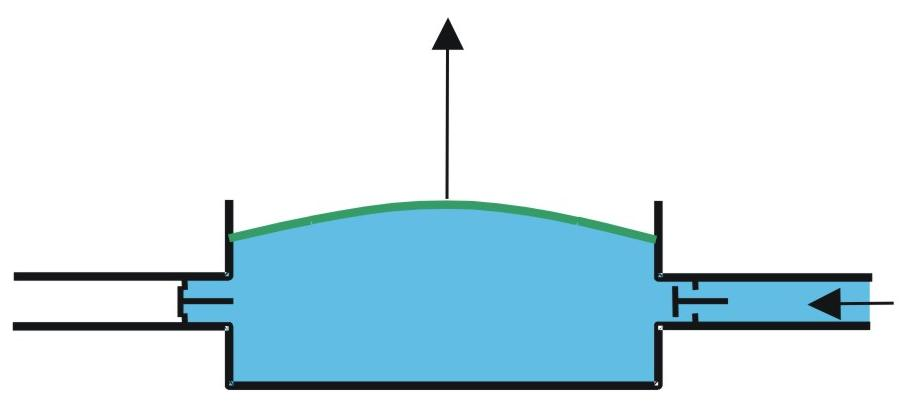
\includegraphics[scale=0.29]{../figs/Bomba_diafragma_aspirando}
\par\end{centering}

}\hfill{}
\par\end{centering}

\caption{Bomba de diafragma.\label{fig:Bomba-de-diafragma}}

\end{figure}


%
\begin{figure}
\begin{centering}
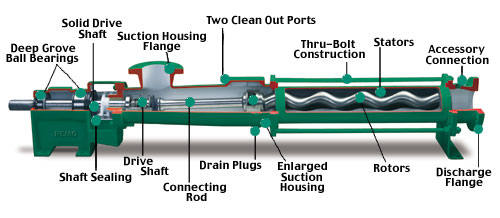
\includegraphics[scale=0.9]{../figs/bombatornillo}
\end{centering}

\caption{Bomba helicoidal.\label{fig:Bomba-helicoidal}}

\end{figure}


Las \emph{bombas rotodinámicas} tienen como principio añadir cantidad
de movimiento. En este tipo de bombas hay uno o varios rodetes con
álabes que giran generando un campo de presiones en el fluido. Dentro
de este grupo son destacables las \emph{bombas radiales o centrífugas}
(figura \ref{fig:Bomba-centr=0000EDfuga}), en las que el fluido entra
por el centro del rodete, que dispone de unos álabes para conducir
el fluido, y por efecto de la fuerza centrífuga es impulsado hacia
el exterior, donde es recogido por la carcasa o cuerpo de la bomba.
El contorno de este cuerpo conduce el fluido hacia las tubuladuras
de salida o hacia el siguiente rodete (también denominado etapa). 

%
\begin{figure}
\begin{centering}
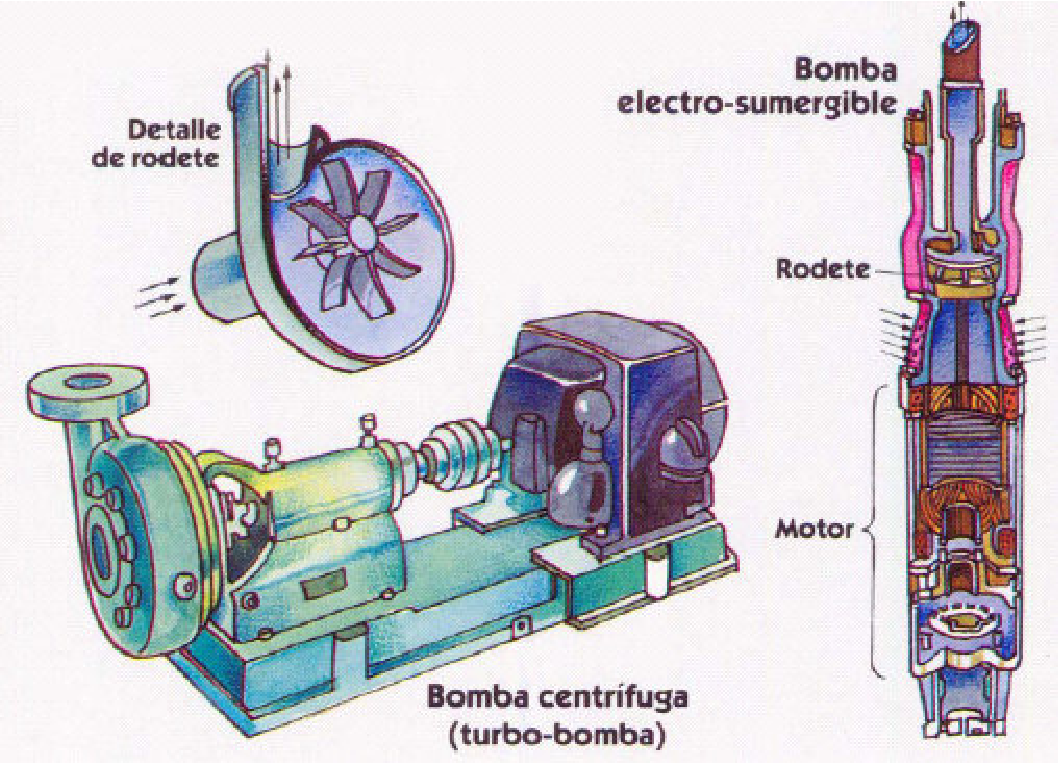
\includegraphics[scale=0.5]{../figs/BombaCentrifuga}
\end{centering}

\caption{Bomba centrífuga de superficie y sumergible.\label{fig:Bomba-centr=0000EDfuga}}

\end{figure}


Las bombas centrífugas están diseñadas para vencer una presión más
o menos constante, proporcionando elevados caudales para bajas alturas
manométricas, y funcionan bien con pequeños pares de arranque. Se
puede aumentar la altura que son capaces de vencer añadiendo etapas
en serie en la misma bomba. Son bombas simples, robustas y de bajo
coste.

Las bombas centrífugas se comportan de acuerdo a las leyes de la semejanza,
según las cuales el caudal es proporcional a la velocidad de giro
(ecuación \ref{eq:SemejanzaCaudal}), la altura es proporcional al
cuadrado de la velocidad (ecuación \ref{eq:SemejanzaAltura}) y la
potencia mecánica en el eje de la bomba (potencia absorbida por la
bomba) es proporcional al cubo de la velocidad (ecuación \ref{eq:SemejanzaPotencia}).
Dado que la potencia mecánica es el producto del par por la velocidad
angular, el par es proporcional al cuadrado de la velocidad (ecuación
\ref{eq:SemejanzaPar}). Estas leyes nos serán útiles para calcular
el cambio en el caudal y altura manométrica de una bomba al variar
su velocidad de giro. La aplicación de estas ecuaciones produce un
punto de trabajo con la misma eficiencia que el correspondiente a
la velocidad de giro original. Dicho de otra forma, estas relaciones
son válidas únicamente cuando se establecen entre puntos de trabajo
con la misma eficiencia.

\begin{center}
\begin{eqnarray}
Q & \propto & n\label{eq:SemejanzaCaudal}\\
H & \propto & n^{2}\label{eq:SemejanzaAltura}\\
P_{mec} & \propto & n^{3}\label{eq:SemejanzaPotencia}\\
T & \propto & n^{2}\label{eq:SemejanzaPar}\end{eqnarray}

\par\end{center}

Según la disposición de la bomba puede distinguirse entre bombas sumergibles,
flotantes y de superficie. Las bombas sumergibles suelen conformar
un único equipo con el motor y son adecuadas para pozos profundos
de pequeño diámetro. Las bombas flotantes son de aplicación en ríos,
lagos o pozos de gran diámetro, lugares con elevado caudal pero escasa
altura manométrica. Finalmente, las bombas de superficie funcionan
por succión a nivel del suelo, facilitando el mantenimiento. Debe
tenerse en cuenta que el nivel de succión es limitado y que, en caso
de utilizar agua como lubricante, no deben operar en seco para evitar
el sobrecalentamiento.


\subsubsection{Configuraciones típicas}

Las cuatro combinaciones de motor eléctrico y bomba de agua más empleadas
en los SFV son la motobomba sumergible con motor AC y bomba centrífuga
multietapa, la bomba sumergible con motor en superficie, la motobomba
flotante con bomba centrífuga, y el motor DC con bomba centrífuga
flotante.

Según la potencia del generador las configuraciones más comunes son:
\begin{itemize}
\item Sistemas de baja potencia (50 a 400 Wp): motor DC accionando una bomba
de membrana y alimentado por un convertidor DC/DC.
\item Sistemas de media potencia (400-1500 Wp):

\begin{itemize}
\item Motobomba con bomba sumergible centrífuga multietapa y motor asíncrono
alimentado por un variador de frecuencia.
\item Motobomba con bomba helicoidal y con motor DC sin escobillas accionado
por un control DC.
\end{itemize}
\item Potencia superior a 1 kWp: motobomba con bomba sumergible centrífuga
multietapa y motor asíncrono alimentado por un variador de frecuencia.
\end{itemize}

\subsection{Acoplamiento generador-motobomba}

Un SFB integra dos equipos cuyo funcionamiento es variable con determinadas
condiciones particulares. Por una parte, el generador fotovoltaico
varía su curva de salida de acuerdo a la irradiancia y a la temperatura.
Por otra, el conjunto motor-bomba cambia de punto de trabajo según
las características de la entrada al motor y según sean las condiciones
del acuífero. Para acoplar adecuadamente estos dos equipos se hace
necesario el uso de un equipo adicional capaz de modificar la señal
de salida del generador para adaptarla a las necesidades de la motobomba,
y también de modificar el punto de trabajo de la motobomba en función
de la potencia disponible en el generador. En los sistemas que emplean
motores de inducción este equipo es un variador de frecuencia, y en
los que incorporan un motor de continúa se trata de un convertidor
DC-DC.


\subsubsection{Convertidor DC-DC}

Un convertidor DC-DC es un dispositivo que transforma corriente continua
de una tensión a otra. En los SFB regulan la tensión de entrada a
la bomba para que el arranque se realice correctamente y la estabilizan
durante el funcionamiento normal. Según sea la relación deseada entre
la tensión de entrada y la tensión de salida se emplea un tipo de
circuito u otro. Por ejemplo, cuando se desea elevar la tensión de
entrada se opta por un circuito tipo \emph{Boost} (figura \ref{fig:Boost}),
pero cuando es necesario que la tensión de salida sea menor que la
de entrada se utiliza un circuito tipo \emph{Buck} (figura \ref{fig:Buck}).
La relación entre la entrada y la salida se puede regular alterando
el ciclo de trabajo del dispositivo de conmutación que incorpora cada
tipo de circuito. 

%
\begin{figure}
\hfill{}\subfloat[Elevador o \emph{Boost.\label{fig:Boost}}]{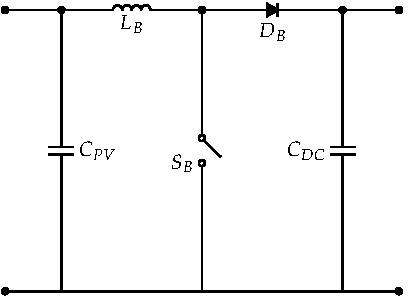
\includegraphics{../figs/Boost}



}\hfill{}\subfloat[Reductor o \emph{Buck.\label{fig:Buck}}]{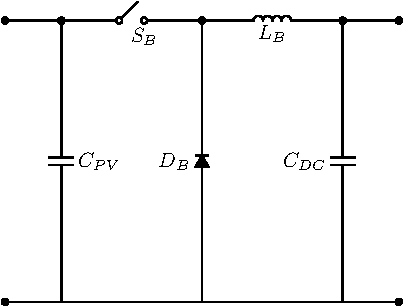
\includegraphics{../figs/Buck}



}\hfill{}

\caption{Convertidores DC-DC.}



\end{figure}



\subsubsection{Variador de frecuencia}

El variador de frecuencia convencional transforma una señal alterna
con una tensión y frecuencia determinadas en otra señal alterna con
otra tensión y frecuencia diferentes. Se compone de un rectificador
y un inversor DC/AC conectados a través de un bus de continua, donde
el rectificador convierte la señal de entrada en continua%
\footnote{En sistemas FV puede evitarse las pérdidas debida al rectificador
conectando directamente al inversor, o bien puede asumirse esta pérdida
y conectar al rectificador, lo que sirve como protección contra inversión
de polaridad. %
}, y el inversor la transforma de nuevo en alterna a la tensión y frecuencia
deseada. 

Este equipo es el encargado de establecer el punto de trabajo al generador
fotovoltaico y a la motobomba de forma que su acoplamiento sea el
adecuado en las condiciones de radiación y temperatura existentes.
Para fijar el punto de trabajo del generador, la práctica habitual
es recurrir a un control PID%
\footnote{El control proporcional-integral-derivativo (PID) es un mecanismo
de control con realimentación ampliamente utilizado en sistemas de
control industrial. Los tres parámetros del algoritmo del control
tiene en cuenta el efecto del error actual (P), el debido a un histórico
de errores recientes (I) y el causado por el ratio de variación del
error (D). Los pesos de una suma ponderada de estos parámetros pueden
ser modificados para ajustar el control.%
} que toma como base una tensión de referencia adaptada al generador
en particular. Es posible incorporar un buscador de MPP aunque su
utilización no es muy frecuente. Para fijar el punto de trabajo de
la motobomba, existen diferentes técnicas de control tales como el
control vectorial o el control tensión-frecuencia o escalar. Nos detendremos
en el control escalar por su frecuente aplicación.

Para comprender la estrategia de funcionamiento del control escalar,
es de particular importancia saber que el par de giro máximo de un
motor de inducción es proporcional al cuadrado del ratio entre la
tensión y la frecuencia de entrada (ecuación \ref{eq:ParCuadraticoMotorInduccion})
\cite{FraileMora2003}:

\begin{equation}
T_{max}=k_{T}\left(\frac{V_{1}}{f_{1}}\right)^{2}\label{eq:ParCuadraticoMotorInduccion}\end{equation}


Junto a esta relación será útil saber que el flujo producido es proporcional
a la fuerza electromotriz que aparece en el estator, $E_{1}$, e inversamente
proporcional a la frecuencia de entrada, $f_{1}$ , según expresa
la ecuación \ref{eq:FemFlujoFrecuenciaEstator}:

\begin{eqnarray}
\phi & = & \frac{E_{1}}{4.44\cdot N_{1}\cdot f_{1}}\label{eq:FemFlujoFrecuenciaEstator}\end{eqnarray}
siendo $N_{1}$ el número de espiras que componen el inductor. Salvo
para bajas frecuencias es posible aproximar la tensión de entrada
a la fuerza electromotriz en el estator, $V_{1}\simeq E_{1}$. Así,
la ecuación \ref{eq:FemFlujoFrecuenciaEstator} se transforma en:

\begin{equation}
\phi\simeq k_{\phi}\frac{V_{1}}{f_{1}}\label{eq:TensionFrecuenciaFlujo}\end{equation}


Por tanto, si la relación entre la tensión y frecuencia de entrada
se mantiene constante, $\frac{V_{1}}{f_{1}}=\mathrm{cte.}$, el
par máximo y el flujo en el entrehierro del motor se mantendrán invariables.
Este modo de control es adecuado para cargas con par constante. Sin
embargo, debe tenerse en cuenta que el par de las bombas centrífugas,
cuando el rendimiento es constante, es proporcional al cuadrado de
la velocidad de giro (ecuación \ref{eq:SemejanzaPar}). Utilizar la
relación anterior para este tipo de cargas no alcanza los valores
de eficiencia óptimos para el conjunto motobomba. Para este tipo de
cargas se han propuesto otros modos de control, desde una modificación
de la curva del control escalar de forma que $V_{1}=k_{V}\cdot f_{1}^{2}$
\cite{Abella.Lorenzo.ea2003,Narvarte.Lorenzo2006}, o métodos más
sofisticados como el control de deslizamiento o el control vectorial
\cite{Bose2002,Bhat.Pittet.ea1987,Correa.Nevesy.ea2008,Famouri.Cathey1991}.

La aproximación realizada en la ecuación \ref{eq:TensionFrecuenciaFlujo}
no es valida a bajas frecuencias. En esta región es necesario aumentar
el valor de la tensión sobre la frecuencia para conseguir que el flujo
magnético en el entrehierro sea el adecuado. Por otra parte, por encima
de la frecuencia nominal, tanto la estrategia de control lineal como
la de control cuadrático obligan a trabajar en tensiones superiores
a la nominal. Dado que no es recomendable superar este umbral, a partir
de este punto la estrategia consiste en mantener constante la tensión
de alimentación del estator y aumentar sólo la frecuencia. De acuerdo
con las ecuaciones \ref{eq:TensionFrecuenciaFlujo} y \ref{eq:ParCuadraticoMotorInduccion},
el flujo y el par máximo disminuirán, pero la potencia permanece constante
con un control adecuado.


\subsection{Protecciones para pozo y depósito}

Durante el funcionamiento del sistema deben evitarse dos situaciones
extremas: el vaciado del pozo y el desbordamiento del depósito.

Cuando la velocidad de extracción de agua por la bomba supera la velocidad
de reposición por el manantial, el giro de la bomba se realizará en
vacío con una mezcla de aire y agua. Este fenómeno, denominado cavitación,
puede dañar la bomba por fricción, vibración excesiva y sobretemperatura.
Un método común para evitar esta situación consiste en controlar la
frecuencia de salida del variador. Cuando la motobomba trabaja en
vacío, la potencia mecánica necesaria baja y con ella la corriente.
Para recuperar la tensión de referencia, el variador debe subir la
frecuencia indefinidamente. Una vez que se alcanza una frecuencia
límite (por ejemplo, $\SI{55}{\hertz}$), esta protección debe ordenar
el paro del sistema. Para permitir que el acuífero sea capaz de reponer
el agua, el control debe incluir un tiempo de espera antes de rearmar
la bomba.

Contra el desbordamiento del depósito caben medidas de aprovechamiento
alternativo del agua. Por ejemplo, puede añadirse una canalización
secundaria que conduzca el agua sobrante para otros usos como regadío,
lavandería, o agua para el ganado. Otro enfoque consiste en detener
la extracción de agua. Este método suele implementarse con la combinación
de un presostato en la tubería y una boya en el depósito. Cuando en
el depósito se alcanza un nivel determinado, la boya acciona el cierre
de la entrada al depósito. Sin embargo, la bomba sigue elevando agua
de forma que la presión dentro de la tubería aumenta hasta accionar
el presostato. Al igual que en la protección contra el vaciado del
pozo, el control debe incluir un tiempo de espera antes de reanudar
la marcha para permitir que baje el nivel del depósito.


\subsection{Circuito hidráulico}

El circuito hidráulico es el conjunto de accesorios que completan
la instalación desde la salida del pozo o sondeo hasta el punto de
suministro, pasando por el almacenaje en depósito elevado en caso
necesario. Comprende elementos tales como la tubería de impulsión,
el depósito elevado, la boca de pozo, la tubería de distribución y
valvulería asociada. 

La tubería de impulsión es la tubería instalada a la salida de la
bomba. Podrá ser de polietileno de alta densidad y calidad alimentaria,
de coste menor pero con ciertos problemas a la hora de la instalación
por su tendencia a enrollarse. Como alternativa están las tuberías
autoportantes flexibles que evitan los problemas anteriores, aunque
su coste es mayor, además de requerir terminales específicos fabricados
en acero inoxidable que encarecen la instalación. 

Para depósitos pequeños ($<\SI{1000}{\litre}$) debe elegirse un depósito
plástico de color negro, ya que los colores que permiten el paso de
la luz favorecen la aparición de algas y otros contaminantes. Este
plástico puede ser polietileno de alta densidad para uso alimentario.


\section{Dimensionado de un SFB}


\subsection{Potencia hidráulica, mecánica y eléctrica en un SFB}

La potencia hidráulica, $P_{H}$, necesaria para bombear agua es función
de la altura vertical aparente, \nomenclature[Ph]{$P_{H}$}{Potencia hidraúlica necesaria en un sistema de bombeo de agua}$H_{v}$\nomenclature[Hv]{$H_{v}$}{Altura vertical aparente en un sistema de bombeo},
y del caudal de agua, $Q$\nomenclature[Q]{$Q$}{Caudal de agua en un sistema de bombeo}:\begin{equation}
P_{H}=g\cdot\rho\cdot Q\cdot H_{v}\label{eq:PotenciaHidraulica}\end{equation}
donde $g$ es la aceleración de la gravedad, y $\rho$ es la densidad
del agua. \nomenclature[g]{$g$}{Aceleración de la gravedad}\nomenclature[rho]{$\rho$}{Densidad del agua}

Expresando $P_{H}$ en watios, $H_{v}$ en metros y $Q$ en $\si{\meter\cubed\per\hour}$
resulta la ecuación \ref{eq:PotenciaHidraulicaUnidades}: \begin{equation}
P_{H}=2.725\cdot Q\cdot H_{V}\label{eq:PotenciaHidraulicaUnidades}\end{equation}


Asumiendo que el agua bombeada sale por el conducto a baja velocidad,
la potencia de salida de la bomba necesita satisfacer $P_{H}$ más
las perdidas de fricción en la tubería, $P_{f}$\nomenclature[Pf]{$P_{f}$}{Pérdidas de fricción en la tubería de un sistema de bombeo}\nomenclature[Hf]{$H_{f}$}{Altura asociada a las pérdidas de fricción en una tubería}.
Este valor se asimila a una altura equivalente $H_{f}$\nomenclature[Ht]{$H_{t}$}{Altura total incluyendo las pérdidas de fricción de la tubería}
asociado a un caudal determinado:\begin{equation}
H_{t}=H_{v}+H_{f}\end{equation}
La potencia eléctrica a la entrada de la motobomba, $P_{el}$, es:\begin{equation}
P_{el}=\frac{P_{H}+P_{f}}{\eta_{mp}}\end{equation}
\nomenclature[Pel]{$P_{el}$}{Potencia eléctrica necesaria en la entrada de una motobomba}donde
$\eta_{mp}$ es la eficiencia de la motobomba.  \nomenclature[etamp]{$\eta_{mp}$}{Eficiencia de una motobomba en un sistema de bombeo}

La potencia eléctrica requerida por la motobomba es entregada por
un generador FV y acondicionada por un acondicionador de potencia:\begin{equation}
P_{el}=P_{g}^{*}\cdot\frac{G}{G_{stc}}\frac{\eta_{g}}{\eta_{g}^{*}}\cdot\eta_{inv}\end{equation}
siendo $G$ la irradiancia en el plano del generador, 
$\eta_{inv}$ la eficiencia del equipo de acondicionamiento
de potencia y $\frac{\eta_{g}}{\eta_{g}^{*}}$ modela el comportamiento
del generador con la temperatura.


\subsection{Cálculo del caudal diario}

El caudal diario bombeado por este conjunto es:\begin{equation}
Q_{d}=\intop_{d}\frac{P_{g}^{*}\cdot\frac{G}{G_{stc}}\frac{\eta_{g}}{\eta_{g}^{*}}\cdot\eta_{inv}\cdot\eta_{mp}}{2.725\cdot H_{T}}\mathrm{dt}\label{eq:CaudalIntegral}\end{equation}
\nomenclature[Qd]{$Q_{d}$}{Caudal diario de agua}

Debido a las variaciones de la temperatura ambiente y de la irradiancia,
y también a causa del comportamiento dinámico de los pozos, todos
los parámetros mencionados anteriormente varían a lo largo del tiempo.
Por tanto, la resolución de la ecuación \ref{eq:CaudalIntegral} no
es tarea evidente. Comprobando el comportamiento de una bomba bajo
distintas condiciones es posible elaborar herramientas gráficas que
resuelven la anterior integral para ciertas condiciones de irradiación
y de temperatura ambiente, siempre considerando constante la altura
total a la que se bombea el agua.

El supuesto de altura total de bombeo constante sólo ocurre cuando,
por un lado, las pérdidas de fricción en la tubería son despreciables
y, cuando por otro, el nivel del agua dentro del pozo se mantiene
constante. Lo primero se puede asegurar usando diámetros de tubería
suficientemente grandes, práctica habitual ya que el elevado coste
de los sistemas de bombeo obliga al uso de sistemas de transporte
y distribución eficientes. De hecho, obtener pérdidas de fricción
por debajo del 5\% de la altura total ($H_{f}<0.05\cdot H_{T}$) constituye
un requisito de optimización de los sistemas fotovoltaicos \cite{Narvarte.Lorenzo2006}.

Se puede definir una {}``altura total equivalente'', $H_{TE}$,
como el hipotético valor constante que llevaría al mismo volumen de
agua bombeada que la ecuación \ref{eq:CaudalIntegral} \cite{Narvarte2001}:

\begin{equation}
Q_{d}=\frac{P_{g}^{*}\cdot}{2.725\cdot G_{stc}\cdot H_{TE}}\cdot\intop_{dia}G\cdot\frac{\eta_{g}}{\eta_{g}^{*}}\cdot\eta_{inv}\cdot\eta_{mp}\mathrm{dt}\label{eq:CaudalHTE}\end{equation}


Ahora, dada una $H_{TE}$, la ecuación \ref{eq:CaudalHTE} depende
exclusivamente de las condiciones meteorológicas y de las características
de la bomba fotovoltaica. 


\subsection{Cálculo de la altura total equivalente}

En la medida de lo posible, es necesario realizar la caracterización
del pozo donde se instalará la bomba. Este ensayo consiste en extraer
agua con una bomba portátil, y medir la caída del nivel del agua en
el pozo a un cierto caudal de bombeo y cuando dicha caída se ha estabilizado.
Tres son los parámetros que completan la caracterización del pozo
tras el ensayo: el nivel estático, $H_{ST}$, el nivel dinámico, $H_{DT}$,
y el caudal de ensayo, $Q_{t}$\nomenclature[Hte]{$H_{TE}$}{Altura total equivalente en un sistema de bombeo}\nomenclature[Hst]{$H_{ST}$}{Nivel estático de un pozo}\nomenclature[Hdt]{$H_{DT}$}{Nivel dinámico de un pozo}\nomenclature[Qt]{$Q_{t}$}{Caudal de ensayo de un pozo}.
Debe tomarse en consideración que la excesiva velocidad de extracción
de agua de un pozo puede dañar su superficie interna y provocar agujeros
que pueden llevar a un eventual colapso del pozo. Consiguientemente,
existe un caudal máximo para cada pozo, $Q_{max}$\nomenclature[Qmax]{$Q_{max}$}{Caudal máximo de extracción de un pozo}.
De hecho, la información de los ensayos mencionados de caracterización
de los pozos están, normalmente, referidos a este caudal máximo al
que se puede extraer el agua de ellos ($Q_{t}=Q_{max}$). 

Con los resultados de este ensayo es posible calcular $H_{TE}$ mediante
\cite{Narvarte2001}:

\begin{equation}
H_{TE}=H_{OT}+H_{ST}+(\frac{H_{DT}-H_{ST}}{Q_{T}})\cdot Q_{AP}+H_{f}(Q_{AP})\end{equation}
donde $H_{OT}$\nomenclature[Hot]{$H_{OT}$}{Diferencia de cotas entre la salida de agua y la entrada en el depósito}
representa la altura desde la salida del pozo hasta la entrada al
depósito y $Q_{AP}$\nomenclature[Qap]{$Q_{AP}$}{Caudal aparente}
el caudal aparente, calculado mediante $Q_{AP}=\alpha\cdot Q_{d}$,
y $\alpha=1 / 24 = \SI[per=reciprocal]{0.0416}{\per\hour}$. El cálculo de las
pérdidas de fricción en función del caudal aparente, $H_{f}(Q_{AP})$,
se realiza recurriendo a las curvas proporcionadas por el fabricante
de las tuberías o fijando un valor constante. En esta ecuación todas
las alturas están expresadas en metros y los caudales en $\si{\meter\cubed\per\hour}$.


\subsection{Procedimiento de dimensionado}
\label{dimensionadoSFB}

Como primera aproximación consideremos constantes a lo largo del
tiempo las eficiencias de los componentes del sistema con la elección
de ciertos valores adecuados ($\frac{\eta_{g}}{\eta_{g}^{*}}=0.85$,
$\eta_{mp}=0.35$, $\eta_{inv}=0.9$). Así, es posible calcular de forma
aproximada la potencia nominal del generador necesaria para bombear un
caudal diario $Q_{d}$ a una altura total equivalente $H_{TE}$ a partir
de la ecuación \ref{eq:CaudalHTE}:

\begin{equation}
  P_{g}^{*}=\frac{10\cdot H_{TE}\cdot Q_{d}}{G_{d}/G_{stc}}
  \label{eq:PotenciaGeneradorBombeo}
\end{equation}
donde $G_d$ es la irradiación global incidente en el plano del generador.

Por ejemplo, para bombear $\SI{30}{\meter\cubed}$ diarios a
$H_{TE}=\SI{40}{\meter}$, con una radiación diaria en el plano del
generador de 
$G_{d}=\SI{5}{\kWh\per\meter\squared}$ se necesita un
generador fotovoltaico de: \[
P_{g}^{*}=\frac{10\cdot40\cdot30}{5}=\SI{2400}{\Wp}\]


Esta primera aproximación nos permite tener un valor de inicio para el
proceso de diseño. A continuación, dividiendo el caudal diario
requerido por la radiación diaria media, se obtiene un número
asimilable a un caudal instantáneo medio
($\si{\meter\cubed\per\hour}$).  Con este caudal, se acude al catálogo
del fabricante elegido%
\footnote{A modo de ejemplo, la nomenclatura de Grundfos para las
  bombas sumergibles es SP-XX-A-YY, siendo XX el caudal instantáneo
  nominal de la bomba e YY un valor relacionado con el número de
  etapas. %
} y se elige un grupo de bombas en el entorno de este caudal
instantáneo medio.  En general, los catálogos de los fabricantes
recogen información del funcionamiento instantáneo de la bomba a su
frecuencia nominal. Por tanto, las curvas H-Q no son de uso inmediato
para el dimensionado de un SFB. Para aproximar el funcionamiento en
frecuencia variable, es recomendable multiplicar el valor de $H_{TE}$
obtenido anteriormente por un factor de $1.4$.

Siguiendo con el ejemplo anterior, la operación $30/5=6$ nos orienta
hacia las bombas SP5 y SP8. En las curvas H-Q de estas bombas situamos
el punto definido por $H=1.4 \cdot 40 = 56$ y $Q=6$, cortando a las
curvas de las bombas SP5A12 y SP8A12.

Con motivo de la ecuación \ref{eq:CaudalIntegral} destacamos la
necesidad de realizar un proceso de simulación del funcionamiento de
la bomba a diferentes frecuencias y su acoplamiento con un generador
bajo diferentes condiciones de radiación y temperatura. El resultado
de este conjunto de simulaciones para cada bomba suele recogerse en
nomogramas o gráficos de doble entrada que relacionan el caudal
diario, la altura total equivalente, la radiación diaria y la potencia
del generador fotovoltaico\footnote{En el apéndice \ref{simulacionSFB}
  se detalla el procedimiento de simulación, implementado en las funciones
\href{http://search.r-project.org/R/library/solaR/html/NmgPVPS.html}{\texttt{NmgSFB}},
\href{http://search.r-project.org/R/library/solaR/html/prodPVPS.html}{\texttt{prodPVPS}} y
\href{http://search.r-project.org/R/library/solaR/html/HQCurve.html}{\texttt{HQCurve}}
de \texttt{solaR} \cite{Perpinan2012b}}.

Con los nomogramas correspondientes al grupo de bombas elegidas de
forma provisional se obtiene un valor más preciso de la potencia del
generador, y se elige la combinación óptima de generador y bomba. Por
ejemplo, la figura \ref{fig:Ejemplo-de-nomograma} recoge un nomograma
elaborado para una bomba Grundfos SP8A44 con una radiación diaria en
el plano del generador de
$\SI{4}{\kWh\per\meter\squared}$.  Si el caudal requerido
fuese de $\SI{30}{\meter\cubed\per\Day}$ y la altura manométrica fuese
de $\SI{125}{\meter}$, el generador fotovoltaico debería tener una
potencia de aproximadamente $\SI{7.5}{\kilo\Wp}$.  Este gráfico
de doble entrada también permite saber el caudal que será capaz de
bombear un generador de una potencia determinada contra una altura
manométrica concreta o en un rango de alturas.

%
\begin{figure}
  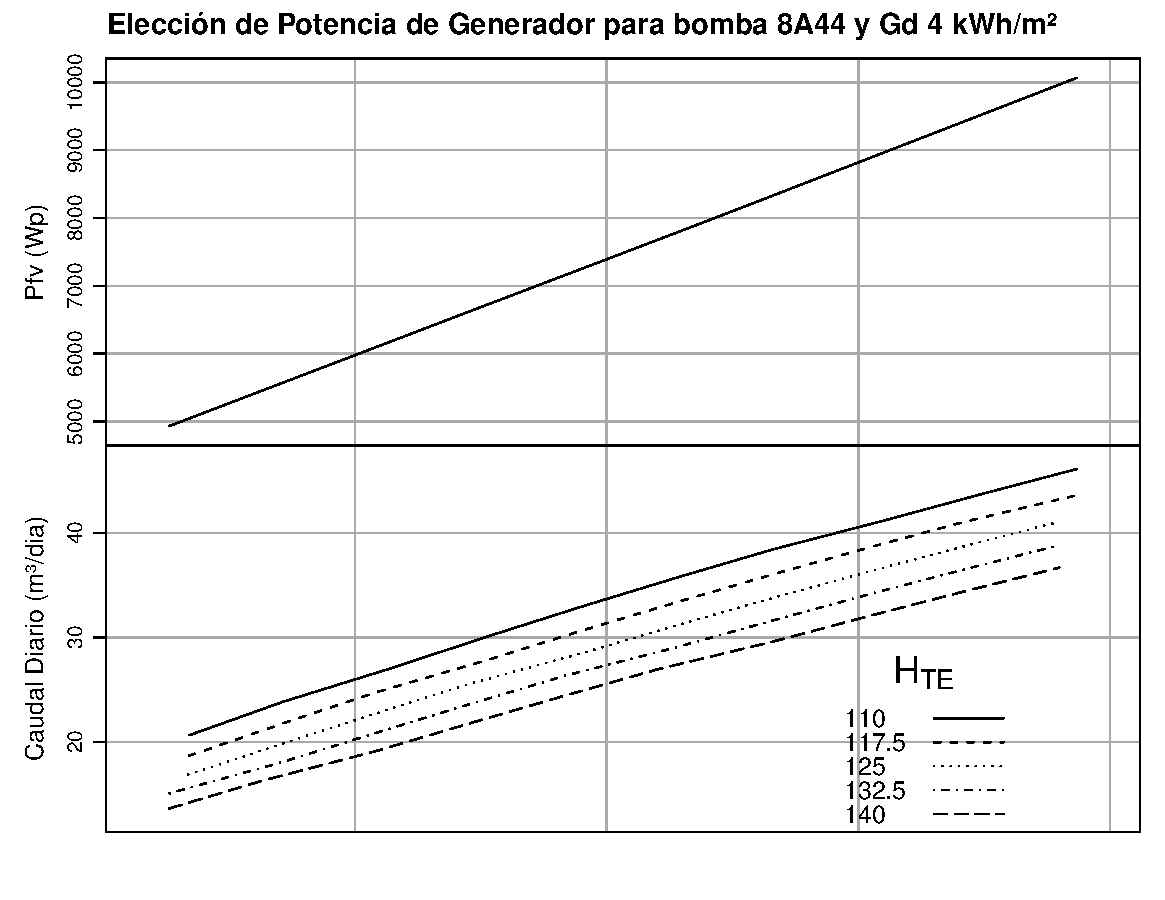
\includegraphics[scale=0.75]{../figs/AbacoBomba}

  \caption[Ejemplo de nomograma para sistemas de bombeo.]{Ejemplo de
    nomograma elaborado para un bomba Grundfos SP8A44 con una
    radiación diaria en el plano del generador
    $\SI{4}{\kWh\per\meter\squared}$.\label{fig:Ejemplo-de-nomograma}
  }



\end{figure}

Es conveniente recurrir a las curvas del fabricante para comprobar el
buen funcionamiento de esta combinación. Así, como seguridad, debe
comprobarse que cuando la potencia entregada por el generador es igual
al 80\% de su potencia nominal, el caudal bombeado correspondiente no
debe exceder el máximo admisible por el pozo.

Una vez decidida la potencia del generador se elige el número de
módulos por serie y el número de ramas. Cuando se emplean variadores
de frecuencia se recomienda que la tensión de entrada al variador sea
al menos:\begin{equation}
  V_{DC}=\frac{\sqrt{2}V_{AC}}{1.1}\end{equation} Así, para una bomba
de tensión de $230\, V_{ac}$ se necesita una tensión en la entrada que
no sea inferior a $300\, V_{dc}$. A partir de esta tensión se
configura el número de módulos por serie y el número de ramas del
generador%
\footnote{Normalmente se ajusta la tensión de entrada al variador de
  forma que sea cercana a la de máxima potencia del generador,
  teniendo en cuenta el efecto de la temperatura. Para hacer un
  cálculo rápido puede tenerse en cuenta que un módulo con 36 células
  en serie ofrece una tensión de $\SI{15}{\volt}$ en este punto cuando
  está en funcionamiento.  Para traducir de forma aproximada este
  número a un módulo con diferente configuración eléctrica puede
  aplicarse una regla de tres.%
}.

Dado que el mayor consumo de agua está localizado en los meses de
verano, conviene emplear un ángulo inferior a la latitud,
$\beta=|\phi|-10^{\circ}$.  En todo caso, la inclinación debe superar
los $15^{\circ}$ para conseguir que la lluvia pueda desplazar la
suciedad acumulada en los paneles.

Finalmente, a partir del caudal $Q_{AP}$ y de la longitud de tubería
necesaria, se elige el diámetro de la misma (mediante las curvas del
fabricante) de forma que las pérdidas sean inferiores a un porcentaje
prefijado de $H_{TE}$.


\subsection{Estimación del caudal}

En el capítulo \ref{tab:Escenarios-de-consumo} discutimos sobre la
incertidumbre asociada a la estimación y predicción del consumo eléctrico.
Lo dicho allí sigue siendo de validez para el problema de estimar
y predecir el caudal consumido en una zona rural. Al igual que allí,
aportaremos unas cifras de contexto que deben ser empleadas con cautela
al ser incorporadas al ejercicio de dimensionado de un SFB. 

La Organización Mundial de la Salud considera que la cantidad diaria
adecuada de agua para consumo humano es de 50 litros por habitante.
En crisis humanitarias, el estándar mínimo es de 3 litros en climas
templados y 5 litros en climas cálidos. En programas de cooperación
se consideran abastecimientos del orden de 30 a 35 litros por persona.
Para sistemas fotovoltaicos, la referencia \cite{Narvarte.Lorenzo2006}
recomienda la cifra de 25 litros por habitante si el suministro se
realiza a través de fuentes comunitarias y 45 litros por habitante
si el suministro se realiza con grifo en cada domicilio.

Frente a estas cifras es útil enfrentar los consumos más cercanos
a nuestra realidad. El consumo en las grandes ciudades se encuentra
hoy en día cerca de los 250 litros por habitante y día. Si se incluyen
todos los consumos, añadiendo los industriales, riego y otros, en
las zonas periféricas con rentas medias más altas y una densidad urbana
menor la dotación media urbana anual se sitúa alrededor de los 350
litros por habitante y día superando los 500 litros para usos globales,
incluyendo el agua urbana, de riego y la destinada a la agricultura.
Estas cantidades están cerca de los 700 litros que cada norteamericano
gasta para lavarse, limpiar el coche o regar.

\section{Simulación de sistemas fotovoltaicos de bombeo}
\label{simulacionSFB}

En la sección \ref{dimensionadoSFB} se ha detallado el procedimiento
de dimensionado de un sistema fotovoltaico de bombeo, y se señalaba la
necesidad de recurrir a métodos de simulación asistidos por
ordenador. En esta sección se amplía la información sobre el algoritmo
necesario y se indican algunas herramientas software que pueden ser
útiles en esta tarea.

Los datos necesarios para la simulación\footnote{El proceso completo
  de simulación está implementado en las funciones
  \href{http://search.r-project.org/R/library/solaR/html/fPump.html}{\texttt{fPump}}
  y
  \href{http://search.r-project.org/R/library/solaR/html/prodPVPS.html}{\texttt{prodPVPS}}
  de \texttt{solaR} \cite{Perpinan2012b}} son:
\begin{itemize}
\item Curvas Altura-Caudal a frecuencia estándar de la bomba elegida preferentemente
realizadas mediante medidas experimentales. 
\item Curvas de rendimiento hidráulico de la bomba centrífuga. 
\item Curvas de rendimiento del motor asíncrono de inducción.
\item Requerimientos del sistema (Altura Manométrica Total, Caudal Diario
Mínimo Requerido)
\item Temperatura ambiente y Radiación Diaria. 
\end{itemize}
El proceso de cálculo es el siguiente:
\begin{enumerate}
\item La curva que relaciona la altura, $H$, y el caudal, $Q$, a la frecuencia
nominal (50 Hz) de la bomba puede trasladarse a otras frecuencias
mediante la curva característica de la bomba: \[
H=a\cdot f^2+b\cdot f\cdot Q+c\cdot Q^2\]
donde $a$, $b$ y $c$ son coeficientes característicos de la
bomba\footnote{Los correspondientes a la gama SP de Grundfos están disponibles en el conjunto de datos \href{http://search.r-project.org/R/library/solaR/html/pumpCoef.html}{\texttt{pumpCoef}}
  de \texttt{solaR} \cite{Perpinan2012b}},
y f la frecuencia considerada. Estos coeficientes pueden calcularse
a partir de las relaciones de semejanza\[
\frac{f_{1}}{f_{2}}=\frac{Q_{1}}{Q_{2}}=\left(\frac{H_{1}}{H_{2}}\right)^{1/2}=\left(\frac{P_{1}}{P_{2}}\right)^{1/3}\]
 validas para las bombas centrífugas. En todos estos puntos el rendimiento
es constante, y por tanto, es posible dibujar una curva de iso-rendimiento
que los une\footnote{Disponible en la función
  \href{http://search.r-project.org/R/library/solaR/html/HQCurve.html}{\texttt{HQCurve}}
  de \texttt{solaR} \cite{Perpinan2012b}}. 
Debe destacarse que la relación de semejanza es aplicable
a la potencia \emph{mecánica} en el eje de la bomba.
\item Esta expresión permite calcular la frecuencia mínima (frecuencia correspondiente
al caudal nulo para las condiciones de altura manométrica del sistema).
Por otra parte, puede calcularse la frecuencia máxima, correspondiente
al caudal máximo de la bomba en cuestión. Entre estos dos valores
se genera un vector de frecuencias ($\vec{f}$)
\item A partir de este vector, considerando altura manométrica constante
(aproximación), se obtiene un vector de caudales ($\vec{Q}$) mediante
la curva característica.
\item Estos valores de caudal corresponden a valores de potencia hidráulica
que debe desarrollar la bomba. Sin embargo, dado que los valores obtenidos
corresponden a frecuencias distintas, se pueden obtener los valores
a la frecuencia nominal utilizando las leyes de la semejanza:\begin{eqnarray*}
Q_{50} & = & 50\cdot\frac{Q}{f}\\
H_{50} & = & H\cdot\left(\frac{50}{f}\right)^{2}\end{eqnarray*}

\item La ecuación de potencia hidráulica es $P_{h,50}=2.725\cdot Q_{50}\cdot H_{50}$. 
\item Utilizando la curva de rendimiento de la bomba a 50 Hz, $\eta_{b}$,
puede calcularse la potencia mecánica que debe entregar el motor en
el eje a la frecuencia nominal.\[
P_{b,50}=P_{h,50}/\eta_{b}\]
 La potencia mecánica a la frecuencia correspondiente puede calcularse
mediante la tercera ley de la semejanza:\[
P_{b}=P_{b,50}\cdot\left(\frac{50}{f}\right)^{3}\]

\item Utilizando la curva de rendimiento del motor a 50 Hz, $\eta_{m}$,
puede calcularse la potencia eléctrica demandada por el mismo para
cada valor de potencia mecánica en eje. Debe realizarse la conversión
$P_{bc}=P_{b}\cdot50/f$, adecuada para un motor asíncrono. Con estos
valores se puede utilizar la curva de rendimiento de motor, $P_{e,50}=P_{bc}/\eta_{m}$,
obteniendo potencias eléctricas demandadas a la frecuencia de 50 Hz.
Nuevamente hay que corregir estos valores con la conversión inversa,
$P_{e}=P_{e,50}\cdot f/50$, para obtener los valores a cada frecuencia
de trabajo.
\item Por último, considerando un rendimiento constante del variador de
frecuencia y pérdidas constantes en el cableado y elementos de conexión,
se calcula la potencia eléctrica en corriente continua necesaria,
$\vec{P}_{dc}$, a cada frecuencia de funcionamiento.
\end{enumerate}
Por tanto, a partir de un vector de frecuencias, $\vec{f}$, se ha
obtenido un vector de potencias DC, $\vec{P}_{dc}$ para una situación
determinada adecuadas a la potencia nominal de la bomba (en torno
al 100\% y 120\% de su motor), y varios vectores intermedios ($\vec{P_{h}}$,
$\vec{P_{b}}$, $\vec{P_{e}}$, etc.) que caracterizan el funcionamiento
del sistema y sus etapas. 

La segunda parte del proceso\footnote{Implementada en la función en la función
  \href{http://search.r-project.org/R/library/solaR/html/NmgPVPS.html}{\texttt{NmgPVPS}}
  de \texttt{solaR} \cite{Perpinan2012b}} consiste en:
\begin{enumerate}
\item Se obtienen valores de irradiancia a través de una base de datos o
de procedimientos de cálculo como el basado en la norma IEC 61725.
Esta norma propone una expresión analítica para calcular el pérfil
de irradiancia correspondiente a un día con irradiación diaria $G_{d}$
($\si{\Wh\per\meter\squared}$) y duración $h=2\cdot t_{0}$,
siendo $t_{0}$ la hora de puesta del sol. Esta expresión es: \[
G=G_{max}\cdot\cos\left(\frac{t}{t_{0}}\cdot\frac{\pi}{2}\right)\cdot\left[1+s\cdot\left\{ 1-\cos\left(\frac{t}{t_{0}}\cdot\frac{\pi}{2}\right)\right\} \right]\]
donde $G$ es la irradiancia ($\si{\watt\per\meter\squared}$)
en la hora $t$, $G_{max}$ es el valor máximo de irradiancia ($\si{\watt\per\meter\squared}$)
durante el día en cuestión, y $s$ es el factor de forma definido
por:\[
s=\frac{d\cdot\frac{\pi}{2}-1}{1-\frac{\pi}{4}}\]
 siendo $d$ el factor de conjunto de datos calculado con:\[
d=\frac{G_{d}}{G_{max}\cdot h}\]

\item Se calcula la potencia producida por un generador fotovoltaico, $P_{fv}$,
a partir de las condiciones de irradiancia y temperatura ambiente.
\item Este valor de potencia debe ser superior a alguno (o todos) los elementos
del vector de potencia $\vec{P}_{dc}$ obtenido anteriormente, obteniendo
un subvector compuesto por todos los elementos inferiores a la potencia
fotovoltaica $P_{fv}$. El elemento mayor de este subvector es el
que utilizaremos como característico del punto de trabajo a una temperatura
y nivel de irradiancia. 
\item Integrando en el tiempo los valores de caudal instantáneo obtenidos
para cada valor de irradiancia se obtiene el valor de caudal diario. 
\end{enumerate}
Realizando esta segunda parte del proceso para cada elemento del vector
de potencias fotovoltaicas, se obtiene una relación entre potencia
instalada y caudal diario que permite elegir la configuración adecuada
para la bomba en cuestión trabajando en unas condiciones determinadas
de radiación, temperatura y altura manométrica. Es habitual presentar
estas combinaciones en forma de gráfico de doble entrada o nomograma
(figura \ref{fig:Ejemplo-de-nomograma}).

La configuración en serie de los paneles suele obligar a instalar
más paneles de los estrictamente necesarios según el proceso descrito.
El valor final de potencia debe introducirse nuevamente en la simulación
para comprobar el correcto funcionamiento de la bomba (para predecir
posibles problemas de sobrefrecuencia y calentamiento).

%%% Local Variables:
%%% mode: LaTex
%%% TeX-master: "ESF.tex"
%%% End: 